\documentclass[a4paper,12pt]{article}

% Packages for language and font settings
\usepackage[utf8]{inputenc}  % For UTF-8 encoding
\usepackage[T1]{fontenc}     % For better font encoding
\usepackage[english]{babel}  % For English language

% Packages for formatting
\usepackage{geometry}        % To customize page layout
\geometry{a4paper, margin=1in}

\usepackage{setspace}        % For line spacing
\onehalfspacing              % Set 1.5 line spacing

\usepackage{parskip}         % Adds space between paragraphs

% Packages for headers and footers
\usepackage{fancyhdr}
\pagestyle{fancy}
\fancyhf{}
\fancyhead[L]{\textbf{Lab Report}} % Left header
\fancyhead[R]{\thepage}            % Right header


% Packages for math and symbols
\usepackage{amsmath, amssymb, amsfonts} % Advanced math
\usepackage{siunitx}                    % For SI units

% Packages for tables and figures
\usepackage{graphicx}                   % For images
\usepackage{caption}                    % For customizing captions
\usepackage{subcaption}                 % For subfigures
\usepackage{booktabs}                   % For professional-quality tables
\usepackage{array}                      % For custom table columns
\usepackage{float}
% Packages for referencing
\usepackage{hyperref}                   % Hyperlinks
\hypersetup{
    colorlinks=true,
    linkcolor=blue,
    citecolor=blue,
    urlcolor=blue,
    pdftitle={Lab Report},
    pdfauthor={Your Name},
}

\usepackage{biblatex}                   % For bibliography management
\addbibresource{references.bib}         % Specify your bibliography file

% Packages for code
\usepackage{listings}                   % Code highlighting
\usepackage{xcolor}                     % Custom colors for listings

\lstset{
    frame=single,
    numbers=left,
    numberstyle=\tiny\color{gray},
    basicstyle=\ttfamily\small,
    keywordstyle=\color{blue},
    stringstyle=\color{red},
    commentstyle=\color{gray},
    breaklines=true,
}

% Custom Commands
\newcommand{\vect}[1]{\mathbf{#1}}      % Shortcut for vectors
\newcommand{\dif}{\mathrm{d}}           % Differential symbol
% Title Page
\title{\textbf{Lab Report 1}}
\author{Suguru Sai Akshita - EE24BTECH11054 \\Sai Akhila Reddy Turpu - EE24BTECH11055 }

\date{\today}

% Begin Document
\begin{document}

\maketitle
\tableofcontents
\newpage

\section{Objective}

1. Observing and analyzing Lissajous figures on a Cathode Ray Oscilloscope (CRO)\\
2. Capturing a one-time event using a CRO

\section{Apparatus and procedure}
\subsection{Materials}
\begin{itemize}
    \item Cathode ray Oscilloscope
    \item Function Generator (2 channels)
    \item Probes
    \item Connecting wires
\end{itemize}

\subsection{Procedure}
\begin{enumerate}
    \item Connect the probe to function generator and turn it off.
    \item Press Mode/Coupling button and then change sweep mode from auto to normal.
    \item In the Trigger menu, press Mode until “Edge” is selected.
    \item Then select Single mode. Wait until mode will initiate.
    \item Turn on the signal and get a captured one-time event.  
\end{enumerate}

\section{Results}
The functions plotted on X and Y axis respectively, are:
\begin{align*}
    V_1(t) &= A_x \sin(2\pi f_x t), \\
    V_2(t) &= A_y \sin(2\pi f_y t + \phi),
\end{align*}
Where:\\
$A_x$ and $A_y$ = Amplitudes of the signals.\\
$f_x$ and $f_y$ = Frequencies.\\
$\phi$ = Phase Difference.\\



\begin{figure}[htbp]
    \centering
    \begin{subfigure}[b]{0.45\textwidth}
        \centering
        \includegraphics[width=\linewidth]{figs/1/plot1.jpeg}
        \caption{Plot}
        \label{fig:image1}
    \end{subfigure}
    \hfill
    \begin{subfigure}[b]{0.45\textwidth}
        \centering
        \includegraphics[width=\linewidth]{figs/1/para1.jpeg}
        \caption{Parameters used}
        \label{fig:image2}
    \end{subfigure}
    \caption{Case 1}
    \label{fig:sidebyside}
\end{figure}


\begin{figure}[htbp]
\begin{center}
    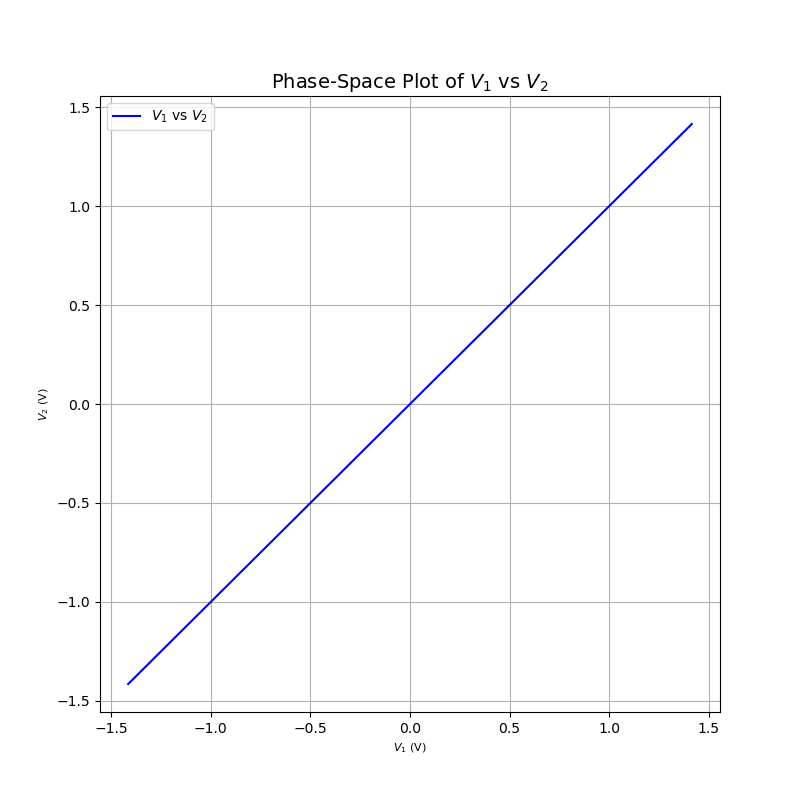
\includegraphics[width=0.7\textwidth]{figs/1/pyplot.png}
\end{center}
\end{figure}


\begin{table}[htbp]
    \centering
    \begin{tabular}{|c|c|c|}
        \hline
        \textbf{Parameter} & \textbf{Value} \\
        \hline
        $V_1(t)$ & \SI{5}{\volt} \\
        $V_2(t)$ & \SI{5}{\volt} \\
        $f_x$ & \SI{1000}{\hertz} \\
        $f_y$ & \SI{1000}{\hertz} \\
        $\phi$ & \SI{0}{\degree} \\
        \hline
    \end{tabular}
    \caption{Data Table}
    \label{tab:sample}
\end{table}



\begin{figure}[htbp]
    \centering
    \begin{subfigure}[b]{0.45\textwidth}
        \centering
        \includegraphics[width=\linewidth]{figs/2/plot2.jpeg}
        \caption{Plot}
        \label{fig:image1}
    \end{subfigure}
    \hfill
    \begin{subfigure}[b]{0.45\textwidth}
        \centering
        \includegraphics[width=\linewidth]{figs/2/para2.jpeg}
        \caption{Parameters used}
        \label{fig:image2}
    \end{subfigure}
    \caption{Case 2}
    \label{fig:sidebyside}
\end{figure}

\begin{figure}[htbp]
\begin{center}
    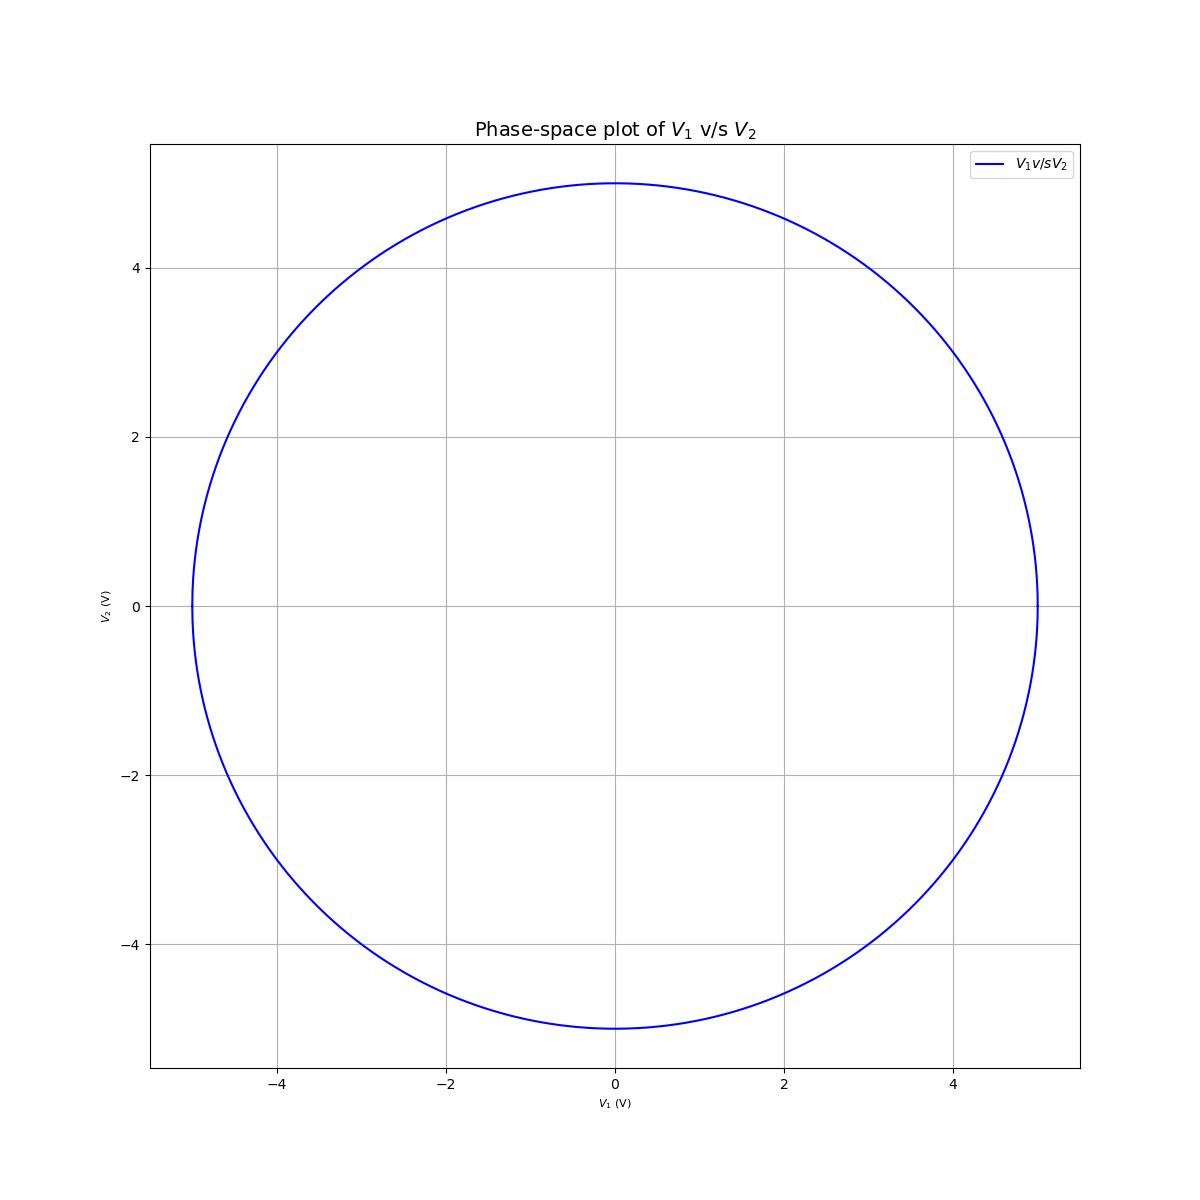
\includegraphics[width=0.7\textwidth]{figs/2/pplot.png}
\end{center}
\end{figure}


\begin{table}[htbp]
    \centering
    \begin{tabular}{|c|c|c|}
        \hline
        \textbf{Parameter} & \textbf{Value} \\
        \hline
        $V_1(t)$ & \SI{5}{\volt} \\
        $V_2(t)$ & \SI{5}{\volt} \\
        $f_x$ & \SI{1000}{\hertz} \\
        $f_y$ & \SI{1000}{\hertz} \\
        $\phi$ & \SI{90}{\degree} \\
        \hline
    \end{tabular}
    \caption{Data Table}
    \label{tab:sample}
\end{table}


\begin{figure}[htbp]
    \centering
    \begin{subfigure}[b]{0.45\textwidth}
        \centering
        \includegraphics[width=\linewidth]{figs/3/plot3.jpeg}
        \caption{Plot}
        \label{fig:image1}
    \end{subfigure}
    \hfill
    \begin{subfigure}[b]{0.45\textwidth}
        \centering
        \includegraphics[width=\linewidth]{figs/3/para3.jpeg}
        \caption{Parameters used}
        \label{fig:image2}
    \end{subfigure}
    \caption{Case 3}
    \label{fig:sidebyside}
\end{figure}

\begin{figure}[htbp]
\begin{center}
    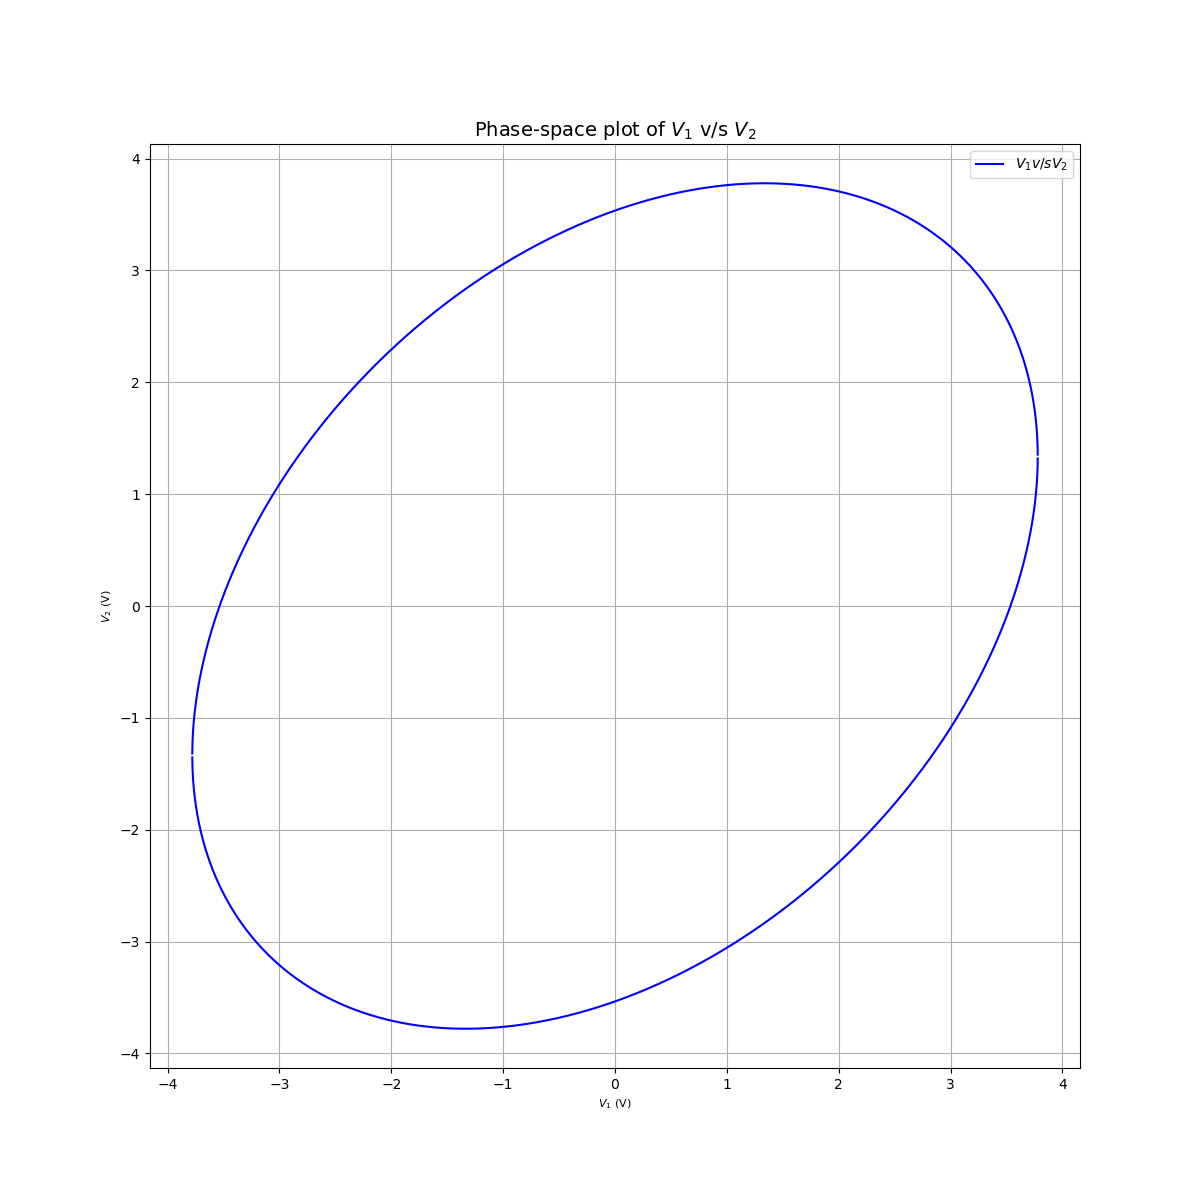
\includegraphics[width=0.7\textwidth]{figs/3/pplot.png}
\end{center}
\end{figure}

\begin{table}[htbp]
    \centering
    \begin{tabular}{|c|c|c|}
        \hline
        \textbf{Parameter} & \textbf{Value} \\
        \hline
        $V_1(t)$ & \SI{5}{\volt} \\
        $V_2(t)$ & \SI{5}{\volt} \\
        $f_x$ & \SI{1000}{\hertz} \\
        $f_y$ & \SI{1000}{\hertz} \\
        $\phi$ & \SI{45}{\degree} \\
        \hline
    \end{tabular}
    \caption{Data Table}
    \label{tab:sample}
\end{table}



\begin{figure}[htbp]
    \centering
    \begin{subfigure}[b]{0.45\textwidth}
        \centering
        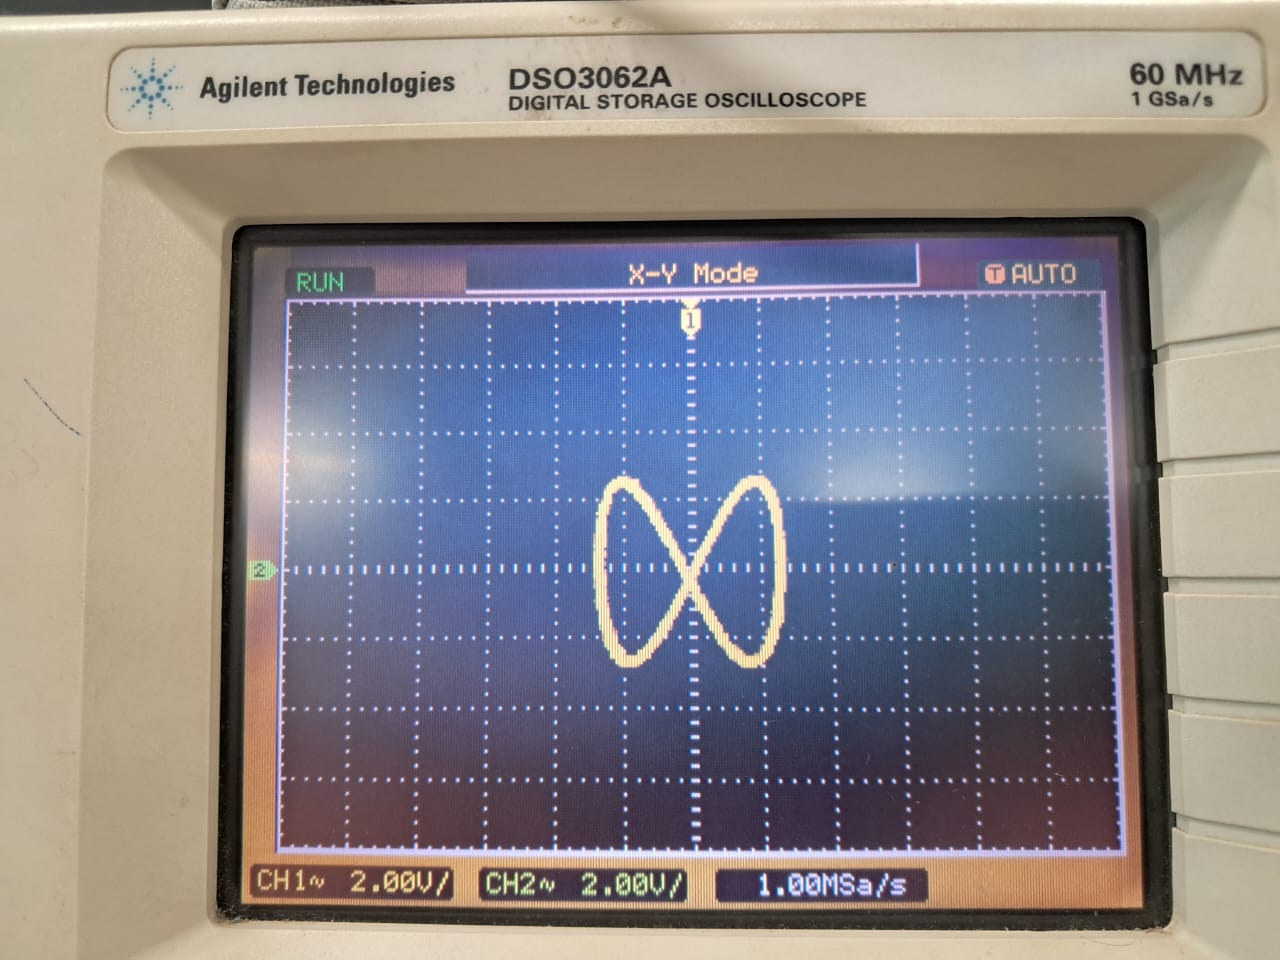
\includegraphics[width=\linewidth]{figs/4/Plot4.jpeg}
        \caption{Plot}
        \label{fig:image1}
    \end{subfigure}
    \hfill
    \begin{subfigure}[b]{0.45\textwidth}
        \centering
        \includegraphics[width=\linewidth]{figs/4/para4.jpeg}
        \caption{Parameters used}
        \label{fig:image2}
    \end{subfigure}
    \caption{Case 4}
    \label{fig:sidebyside}
\end{figure}

\begin{figure}[htbp]
\begin{center}
    \includegraphics[width=0.7\textwidth]{figs/4/pplot.png}
\end{center}
\end{figure}


\begin{table}[htbp]
    \centering
    \begin{tabular}{|c|c|c|}
        \hline
        \textbf{Parameter} & \textbf{Value} \\
        \hline
        $V_1(t)$ & \SI{5}{\volt} \\
        $V_2(t)$ & \SI{5}{\volt} \\
        $f_x$ & \SI{100}{\hertz} \\
        $f_y$ & \SI{200}{\hertz} \\
        $\phi$ & \SI{0}{\degree} \\
        \hline
    \end{tabular}
    \caption{Data Table}
    \label{tab:sample}
\end{table}



\begin{figure}[htbp]
    \centering
    \begin{subfigure}[b]{0.45\textwidth}
        \centering
        \includegraphics[width=\linewidth]{figs/5/plot5.jpeg}
        \caption{Plot}
        \label{fig:image1}
    \end{subfigure}
    \hfill
    \begin{subfigure}[b]{0.45\textwidth}
        \centering
        \includegraphics[width=\linewidth]{figs/5/para5.jpeg}
        \caption{Parameters used}
        \label{fig:image2}
    \end{subfigure}
    \caption{Case 5}
    \label{fig:sidebyside}
\end{figure}

\begin{figure}[htbp]
\begin{center}
    \includegraphics[width=0.7\textwidth]{figs/5/pplot.png}
\end{center}
\end{figure}


\begin{table}[htbp]
    \centering
    \begin{tabular}{|c|c|c|}
        \hline
        \textbf{Parameter} & \textbf{Value} \\
        \hline
        $V_1(t)$ & \SI{5}{\volt} \\
        $V_2(t)$ & \SI{5}{\volt} \\
        $f_x$ & \SI{100}{\hertz} \\
        $f_y$ & \SI{100}{\hertz} \\
        $\phi$ & \SI{180}{\degree} \\
        \hline
    \end{tabular}
    \caption{Data Table}
    \label{tab:sample}
\end{table}


\begin{figure}[htbp]
    \centering
    \begin{subfigure}[b]{0.45\textwidth}
        \centering
        \includegraphics[width=\linewidth]{figs/6/plot6.jpeg}
        \caption{Plot}
        \label{fig:image1}
    \end{subfigure}
    \hfill
    \begin{subfigure}[b]{0.45\textwidth}
        \centering
        \includegraphics[width=\linewidth]{figs/6/para6.jpeg}
        \caption{Parameters used}
        \label{fig:image2}
    \end{subfigure}
    \caption{Case 6}
    \label{fig:sidebyside}
\end{figure}

\begin{figure}[htbp]
\begin{center}
    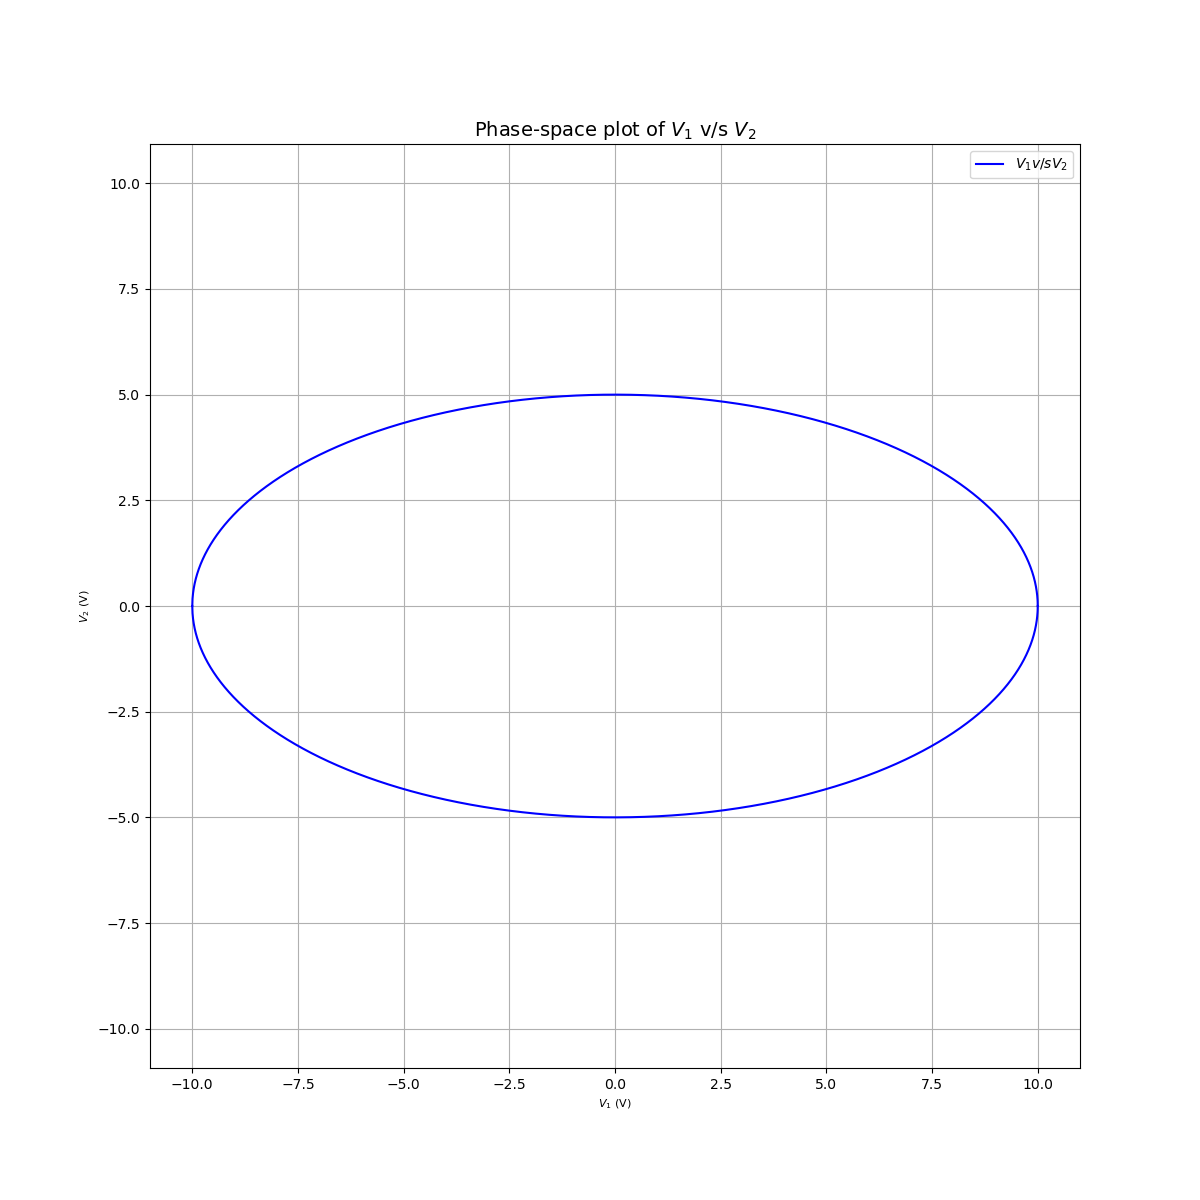
\includegraphics[width=0.7\textwidth]{figs/6/pplot.png}
\end{center}
\end{figure}


\begin{table}[htbp]
    \centering
    \begin{tabular}{|c|c|c|}
        \hline
        \textbf{Parameter} & \textbf{Value} \\
        \hline
        $V_1(t)$ & \SI{10}{\volt} \\
        $V_2(t)$ & \SI{5}{\volt} \\
        $f_x$ & \SI{100}{\hertz} \\
        $f_y$ & \SI{100}{\hertz} \\
        $\phi$ & \SI{90}{\degree} \\
        \hline
    \end{tabular}
    \caption{Data Table}
    \label{tab:sample}
\end{table}





\section{Theory}

\subsection{Case 1:}
\begin{align*}
    &V_1=5\sin(2\pi 1000t)V\\
    &V_2=5\sin(2\pi 1000t)V\\
    &V_1=V_2
\end{align*}


\subsection{Case 2:}
\begin{align*}
    &V_1=\sqrt{2}\sin(2\pi 5000t)V\\
    &V_2=\sqrt{2}\cos(2\pi 5000t)V\\
    &V_1^2+V_2^2=25
\end{align*}

\subsection{Case 3:}

\begin{align*}
    &V_1=5\sin(2\pi 1000t)V\\
    &V_2=5\sin(2\pi 1000t+\frac{\pi}{4})V\\
    &2V_1^2+2V_2^2-\sqrt{2}V_1V_2=25
\end{align*}
\subsection{Case 4:}
\begin{align*}
    &V_1=5\sin(2\pi 100t)V\\
    &V_2=5\sin(2\pi 200t)V\\
    &V_2=2V_1(\sqrt{1-\frac{V_1^2}{25}})
\end{align*}


\subsection{Case 5:}
\begin{align*}
    &V_1=5\sin(2\pi 100t)V\\
    &V_2=5\sin(2\pi 100t+\pi )V\\
    &V_1=-V_2
\end{align*}



\subsection{Case 6:}
\begin{align*}
    &V_1=10\sin(2\pi 100t)V\\
    &V_2=5\sin(2\pi 100t+\frac{\pi}{2})V\\
    &\frac{V_1^2}{100}+\frac{V_2^2}{25}=1
\end{align*}


\section{Capturing One time event Using CRO}
\subsection{Procedure}
\begin{enumerate}
    \item Connect probe to signal generator and then turn it off.
    \item Press Mode/Coupling and change sweep mode from Auto to Normal.
    \item In the Trigger menu, press Mode until “Edge” is selected.
    \item Now press Single mode. After that wait mode will initiate.
    \item Next, Turn on the signal and get a captured one-time event.  
\end{enumerate}

\subsection{Plots}
\begin{figure}[htbp]
    \centering
    \begin{subfigure}[b]{0.45\textwidth}
        \centering
        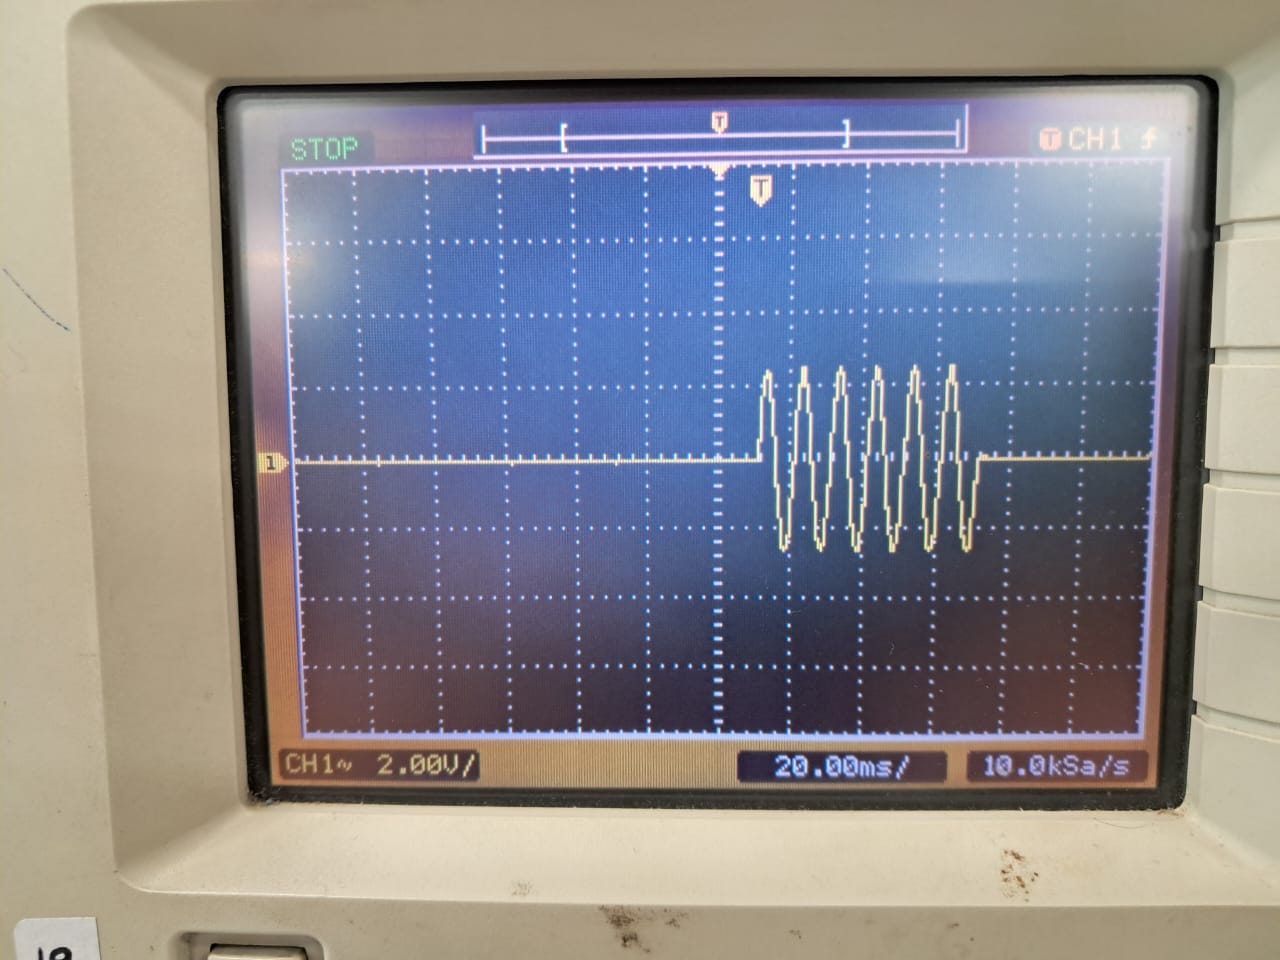
\includegraphics[width=\linewidth]{figs/onetimeplot.jpeg}
        \caption{Plot}
        \label{fig:image1}
    \end{subfigure}
    \hfill
    \begin{subfigure}[b]{0.45\textwidth}
        \centering
        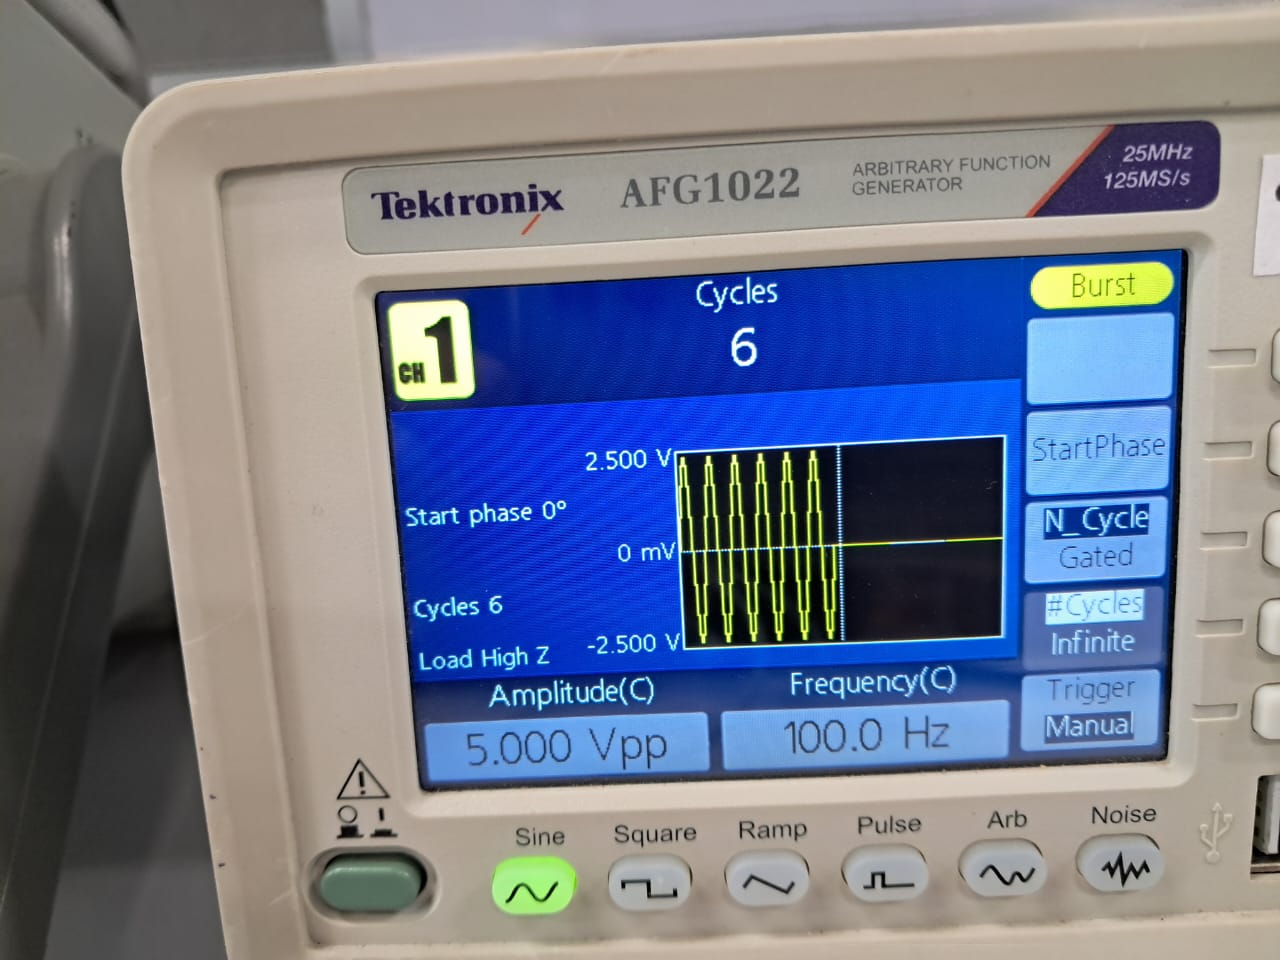
\includegraphics[width=\linewidth]{figs/onetime.jpeg}
        \caption{Parameters used}
        \label{fig:image2}
    \end{subfigure}
    \caption{Plot for One time event}
    \label{fig:sidebyside}
\end{figure}



\end{document}
